\section{Adaptive Komponente in Hadoop}\label{sec:inriaSetting}

Eine normale Hadoop-Installation besitzt keine adaptive Komponente, sondern rein statische Einstellungen. Um damit Hadoop zu optimieren, müssen die Einstellungen immer manuell auf den jeweils benötigten Anwendungstyp angepasst werden. Dazu gibt es auch bereits verschiedene Scheduler, den \emph{Fair Scheduler}, welcher alle Anwendungen ausführt und ihnen gleich viele Ressourcen zuteilt, und den \emph{Capacity Scheduler}. Letzterer sorgt dafür, dass nur eine bestimmte Anzahl an Anwendungen pro Benutzter gleichzeitig ausgeführt wird und teilt ihnen so viele Ressourcen zu, wie benötigt werden bzw. der Benutzter nutzen darf. Entwickelt wurde der Capacity Scheduler vor allem für Cluster, die von mehreren Organisationen gemeinsam verwendet werden und sicherstellen soll, dass jede Organisation eine Mindestmenge an Ressourcen zur Verfügung hat \cite{HadoopCapScheduler271}.

Je nach Bedarf besitzt der Capacity Scheduler entsprechende Einstellungen, um \zB den verfügbaren Speicher pro Container festzulegen. Eine weitere Einstellung des Schedulers ist \acl{MARP}, auch \acs{MARP} gennant\acused{MARP}, der angibt, wie viele Prozent der gesamten Ressourcen durch \ac{AppMstr}-Container genutzt werden dürfen \cite{HadoopCapScheduler271}. Damit bewirkt diese Einstellung indirekt auch die maximale Anzahl an Anwendungen, die gleichzeitig ausgeführt werden dürfen. Da der \ac{MARP}-Wert jedoch nicht während der Laufzeit dynamisch angepasst werden kann, haben \citeauthor{zhang2016} in \cite{zhang2016} einen Ansatz zur dynamischen Anpassung des \ac{MARP}-Wertes zur Laufzeit von Hadoop vorgestellt. Dadurch wird der \ac{MARP}-Wert abhängig von den ausgeführten Anwendungen adaptiv zur Laufzeit angepasst, sodass immer möglichst viele Anwendungen gleichzeitig ausgeführt werden können. Gemäß \citeauthor{zhang2016} werden dadurch Anwendungen im Schnitt um bis zu 40 \% schneller ausgeführt.

\begin{figure}
    \centering
    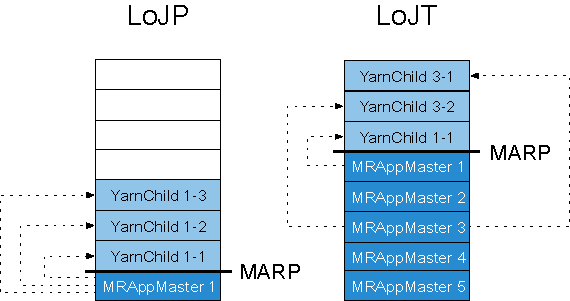
\includegraphics[width=.8\columnwidth]{./images/marpValue.pdf}
    \caption[LoJP und LoJT in Hadoop]{LoJP und LoJT in Hadoop \cite{zhang2016}}
    \label{fig:marpValue}
\end{figure}

Der Hintergrund dieser \emph{Selfbalancing-Komponente} ist der, dass durch den \ac{MARP}-Wert der für die Anwendungen verfügbare Speicher in zwei Teile aufgeteilt wird. Im einen Teil befinden sich alle derzeit ausgeführten \ac{AppMstr}, im anderen Teil die von den Anwendungen benötigten weiteren Container. Wie groß der Teil für die \ac{AppMstr} ist, wird nun durch den \ac{MARP}-Wert bestimmt. Ist der \ac{MARP}-Wert zu klein, können nur wenige \ac{AppMstr} (und damit Anwendungen) gleichzeitig ausgeführt werden (\emph{Loss of Jobs Parallelism}, LoJP). Ist der \ac{MARP}-Wert jedoch zu groß, können für die ausgeführten Anwendungen nur wenige Container bereitgestellt werden, wodurch sich die Ausführung für eine Anwendung wesentlich verlangsamt (\emph{Loss of Job Throughput}, LoJT)\cite{zhang2016}.

Die Selfbalancing-Komponente passt daher den \ac{MARP}-Wert abhängig von der Speicherauslastung dynamisch zur Laufzeit an. So wird der \ac{MARP}-Wert verringert, wenn die Speicherauslastung sehr hoch ist, und erhöht, wenn die Speicherauslastung sehr niedrig ist \cite{zhang2016}. Dadurch wird es ermöglicht, dass die maximal mögliche Anzahl an Anwendungen ausgeführt werden kann. Die Evaluation von \citeauthor{zhang2016} ergab zudem, dass die dynamische Anpassung des \ac{MARP}-Wertes zudem auch effizienter ist als eine manuelle, statische Optimierung.
